\documentclass[pdf]{beamer}
\usepackage[english,vietnamese]{babel}
\usepackage{amsmath}
\usepackage{booktabs}
\usepackage{colortbl}
\usepackage{graphicx}
\usepackage{hyperref}
\usepackage{lmodern}
\usepackage{forest}

\mode<presentation>{}
\usetheme[hideothersubsections]{Hannover}
\usefonttheme[onlymath]{serif}
\usebackgroundtemplate{
  
\includegraphics[width=\paperwidth,height=\paperheight]{USTH.jpg}}
\beamerdefaultoverlayspecification{<+->}

\title[Sort \& Search]{Sorting and Searching}
\author[Group 11]{Nguyễn Công Thành---BI9-210\\
                  Nguyễn Gia Phong---BI9-184\\
                  Nguyễn Văn Tùng---BI9-229\\
                  Trần Minh Vương---BI9-239\\
                  Trần Hồng Minh---BI8-114}
\institute{University of Science and Technology of Hà Nội}
\date{\selectlanguage{english}\today}

\begin{document}
\frame{\titlepage}
\begin{frame}{Contents}
  \tableofcontents
\end{frame}

\section{Introduction}
\begin{frame}{Introduction}\Large
  \begin{itemize}
    \item Sorting \& Searching are \emph{important}
    \item Object-Oriented Programming
    \item Implementation in Java
    \item Generic Programming
  \end{itemize}
\end{frame}

\section{Searching}
\begin{frame}[fragile]{Searching}\Large
  Given a value $x$, return the [zero-based] index of $x$ in the array,
  if such $x$ exists.  Otherwise, return \verb|NOT_FOUND| (-1).
\end{frame}

\subsection{Linear Search}
\begin{frame}[fragile]{Linear Search}\Large
  \begin{itemize}
    \item Checks sequentially till
      \begin{itemize}\Large
        \item match found
        \item whole list searched
      \end{itemize}
    \item Linear time complexity
    \item \verb|java.util.List.indexOf|
    \item Example: Search for number 7
      \begin{center}
        \only<1-5>{\begin{tabular}{|c|c|c|c|c|}
          \hline 4 & 20 & 6 & 9\\\hline
        \end{tabular}}%
        \only<6>{\begin{tabular}{|c|c|c|c|c|}
          \hline \cellcolor{yellow}4 & 20 & 6 & 9\\\hline
        \end{tabular}}%
        \only<7>{\begin{tabular}{|c|c|c|c|c|}
          \hline 4 & \cellcolor{yellow}20 & 6 & 9\\\hline
        \end{tabular}}%
        \only<8>{\begin{tabular}{|c|c|c|c|c|}
          \hline 4 & 20 & \cellcolor{yellow}6 & 9\\\hline
        \end{tabular}}%
        \only<9>{\begin{tabular}{|c|c|c|c|c|}
          \hline 4 & 20 & 6 & \cellcolor{yellow}9\\\hline
        \end{tabular}}
      \end{center}
  \end{itemize}
\end{frame}

\begin{frame}[fragile]{Implementation}
\begin{verbatim}
import java.util.List;

public class Search
{
  public static final int NOT_FOUND = -1;

  public static linear(List l, Object o)
  {
    for (int i = 0; i < l.size(); ++i)
      if (o == null ? l.get(i) == null
                    : o.equals(l.get(i)))
        return i;
    return NOT_FOUND;
  }
}
\end{verbatim}
\end{frame}

\subsection{Binary Search}
\begin{frame}[fragile]{Binary Search}\Large
  \begin{itemize}
    \item For sorted arrays only
    \item Repeat halving interval cannot have $x$ till
      \begin{itemize}\Large
        \item match found
        \item invalid interval
      \end{itemize}
    \item Logarithmic time complexity
    \item \verb|java.util.Collections.binarySearch|
    \item Example: Search for number 7
      \begin{center}
        \only<1-6>{\begin{tabular}{|c|c|c|c|c|c|c|c|c|c|c|}
          \hline 0 & 1 & 2 & 3 & 4 & 5 & 6 & 7 & 8 & 9 & $\emptyset$\\\hline
        \end{tabular}}%
        \only<7>{\begin{tabular}{|c|c|c|c|c|c|c|c|c|c|c|}
          \hline \cellcolor{red}0 & 1 & 2 & 3 & 4 & \cellcolor{green}5
          & 6 & 7 & 8 & 9 & \cellcolor{blue}$\emptyset$\\\hline
        \end{tabular}}%
        \only<8>{\begin{tabular}{|c|c|c|c|c|c|c|c|c|c|c|}
          \hline 0 & 1 & 2 & 3 & 4 & 5 & \cellcolor{red}6 & 7
          & \cellcolor{green}8 & 9 & \cellcolor{blue}$\emptyset$\\\hline
        \end{tabular}}%
        \only<9>{\begin{tabular}{|c|c|c|c|c|c|c|c|c|c|c|}
          \hline 0 & 1 & 2 & 3 & 4 & 5 & \cellcolor{yellow}6 & \cellcolor{blue}7
          & 8 & 9 & $\emptyset$\\\hline
        \end{tabular}}%
        \only<10>{\begin{tabular}{|c|c|c|c|c|c|c|c|c|c|c|}
          \hline 0 & 1 & 2 & 3 & 4 & 5 & 6 & \cellcolor{gray}7
          & 8 & 9 & $\emptyset$\\\hline
        \end{tabular}}
      \end{center}
  \end{itemize}
\end{frame}

\begin{frame}[fragile]{Implementation}
\begin{verbatim}
public class Search
{
  private static <T> int binary(
    List<? extends Comparable<? super T>> list,
    T key, int low, int high)
  {
    if (high < low)
      return NOT_FOUND;
    var mid = (low + high) / 2;
    var cmp = list.get(mid).compareTo(key);
    if (cmp < 0)
      return binary(list, key, mid + 1, high);
    if (cmp > 0)
      return binary(list, key, low, mid - 1);
    return mid;
  }
}
\end{verbatim}
\end{frame}

\begin{frame}[fragile]{Wrapper}
\begin{verbatim}
public class Search
{
  public static <T> int binary(
    List<? extends Comparable<? super T>> list,
    T key)
  {
    return binary(list, key, 0, list.size());
  }
}
\end{verbatim}
\end{frame}

\section{Sorting}
\begin{frame}{Sorting}\Large
  Given an array of $n$ values, arrange the values into ascending order.
\end{frame}

\subsection{Selection Sort}
\begin{frame}{Selection Sort}\Large
  \begin{itemize}
    \item Iterate through every position,\\
      select the minimum from there to array's end
    \item Quadratic time complexity
    \item Example:
      \only<1-2>{\begin{tabular}{|c|c|c|c|c|}
        \hline 6 & 9 & 4 & 2 & 0\\\hline
      \end{tabular}}%
      \only<3>{\begin{tabular}{|c|c|c|c|c|}
        \hline 6 & 9 & 4 & 2 & \cellcolor{yellow}0\\\hline
      \end{tabular}}%
      \only<4>{\begin{tabular}{|c|c|c|c|c|}
        \hline \cellcolor{gray}0 & 9 & 4 & \cellcolor{yellow}2 & 6\\\hline
      \end{tabular}}%
      \only<5>{\begin{tabular}{|c|c|c|c|c|}
        \hline \cellcolor{gray}0 & \cellcolor{gray}2 &
        \cellcolor{yellow}4 & 9 & 6\\\hline
      \end{tabular}}%
      \only<6>{\begin{tabular}{|c|c|c|c|c|}
        \hline \cellcolor{gray}0 & \cellcolor{gray}2 &
        \cellcolor{gray}4 & 9 & \cellcolor{yellow}6\\\hline
      \end{tabular}}%
      \only<7>{\begin{tabular}{|c|c|c|c|c|}
        \hline \cellcolor{gray}0 & \cellcolor{gray}2 &
        \cellcolor{gray}4 & \cellcolor{gray}6 & \cellcolor{yellow}9\\\hline
      \end{tabular}}%
      \only<8>{\begin{tabular}{|c|c|c|c|c|}
        \hline\rowcolor{gray} 0 & 2 & 4 & 6 & 9\\\hline
      \end{tabular}}
  \end{itemize}
\end{frame}

\begin{frame}[fragile,label=selimpl]{Implementation}
\begin{verbatim}
import static java.util.Collections.swap;

public class Sort
{
  public static <T extends Comparable<? super T>>
  void selection(List<T> list)
  {
    int i, j, m, n = list.size();
    for (i = 0; i < n; ++i)
      {
        for (m = j = i; j < n; ++j)
          if (list.get(j).compareTo(list.get(m)) < 0)
            m = j;
        swap(list, i, m);
      }
  }
}
\end{verbatim}
\end{frame}

\subsection{Bubble Sort}
\begin{frame}{Bubble Sort}\Large
  \begin{itemize}
    \item Repeatedly iterate through the array,\\
      swap adjacent elements in wrong order
    \item Quadratic time complexity
    \item Example:
      \only<1-2>{\begin{tabular}{|c|c|c|c|c|}
        \hline 6 & 9 & 4 & 2 & 0\\\hline
      \end{tabular}}%
      \only<3>{\begin{tabular}{|c|c|c|c|c|}
        \hline \cellcolor{magenta}6 & \cellcolor{yellow}9 & 4 & 2 & 0\\\hline
      \end{tabular}}%
      \only<4>{\begin{tabular}{|c|c|c|c|c|}
        \hline 6 & \cellcolor{magenta}9 & \cellcolor{yellow}4 & 2 & 0\\\hline
      \end{tabular}}%
      \only<5>{\begin{tabular}{|c|c|c|c|c|}
        \hline 6 & 4 & \cellcolor{magenta}9 & \cellcolor{yellow}2 & 0\\\hline
      \end{tabular}}%
      \only<6>{\begin{tabular}{|c|c|c|c|c|}
        \hline 6 & 4 & 2 & \cellcolor{magenta}9 & \cellcolor{yellow}0\\\hline
      \end{tabular}}%
      \only<7>{\begin{tabular}{|c|c|c|c|c|}
        \hline \cellcolor{magenta}6 & \cellcolor{yellow}4
        & 2 & 0 & \cellcolor{gray}9\\\hline
      \end{tabular}}%
      \only<8>{\begin{tabular}{|c|c|c|c|c|}
        \hline 4 & \cellcolor{magenta}6 & \cellcolor{yellow}2
        & 0 & \cellcolor{gray}9\\\hline
      \end{tabular}}%
      \only<9>{\begin{tabular}{|c|c|c|c|c|}
        \hline 4 & 2 & \cellcolor{magenta}6 & \cellcolor{yellow}0
        & \cellcolor{gray}9\\\hline
      \end{tabular}}%
      \only<10>{\begin{tabular}{|c|c|c|c|c|}
        \hline \cellcolor{magenta}4 & \cellcolor{yellow}2 & 0
        & \cellcolor{gray}6 & \cellcolor{gray}9\\\hline
      \end{tabular}}%
      \only<11>{\begin{tabular}{|c|c|c|c|c|}
        \hline 2 & \cellcolor{magenta}4 & \cellcolor{yellow}0
        & \cellcolor{gray}6 & \cellcolor{gray}9\\\hline
      \end{tabular}}%
      \only<12>{\begin{tabular}{|c|c|c|c|c|}
        \hline \cellcolor{magenta}2 & \cellcolor{yellow}0
        & \cellcolor{gray}4 & \cellcolor{gray}6 & \cellcolor{gray}9\\\hline
      \end{tabular}}%
      \only<13>{\begin{tabular}{|c|c|c|c|c|}
        \hline\rowcolor{gray} 0 & 2 & 4 & 6 & 9\\\hline
      \end{tabular}}
  \end{itemize}
\end{frame}

\begin{frame}[fragile]{Implementation}
\begin{verbatim}
public class Sort
{
  public static <T extends Comparable<? super T>>
  void bubble(List<T> list)
  {
    for (int n = list.size(), m = 0;
         n > 1; n = m, m = 0)
      for (int i = 1; i < n; ++i)
        if (list.get(i).compareTo(list.get(i-1)) < 0)
          swap(list, m = i, i - 1);
  }
}
\end{verbatim}
\end{frame}

\begin{frame}{Bubble v Selection: Dawn of Sort}\Large
  \only<1>{
    C. Thomas Wu (2010) claimed that
    \begin{quote}
      On average, we expect the bubble sort to finish sorting sooner than
      the selection sort, \emph{because there will be more data movements for
      the same number of comparisons}, and there is a test to exit the method
      when the array gets sorted.
    \end{quote}}
  \only<2>{
\includegraphics[width=\textwidth]{squint.jpg}}
\end{frame}

\begin{frame}{BvS: Time Complexity}
  \begin{center}
    \begin{tabular}{c c c c c}
      \toprule
      Case & \multicolumn{2}{c}{Selection Sort}
           & \multicolumn{2}{c}{Bubble Sort}\\
      \midrule
      & Comparisons & Swaps & Comparisons & Swaps\\
      Best & $\Omega(n^2)$ & $\Omega(n)$ & $\Omega(n)$ & $\Omega(n)$\\
      Average & $\Theta(n^2)$ & $\Theta(n)$ & $\Theta(n^2)$ & $\Theta(n^2)$\\
      Worst & $O(n^2)$ & $O(n)$ & $O(n^2)$ & $O(n^2)$\\
      \bottomrule
    \end{tabular}
  \end{center}
\end{frame}

\begin{frame}{BvS: Average Case in Practice}
  \begin{center}
    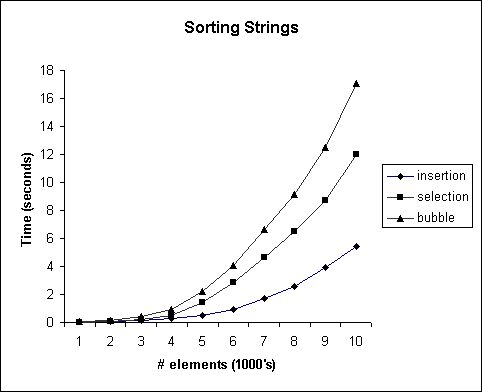
\includegraphics[width=0.85\textwidth]{bubbleplot.jpg}
  \end{center}
\end{frame}

\subsection{Heapsort}
\begin{frame}{Heapsort}\Large
  \begin{itemize}
    \item Selection sort, but use heap for selection
    \item Linearithmic time complexity
  \end{itemize}
\end{frame}

\begin{frame}[fragile]{Using PriorityQueue (Min-Heap)}
\begin{verbatim}
import java.util.PriorityQueue;

public class Sort
{
  public static <T extends Comparable<? super T>>
  void pq(List<T> list)
  {
    var q = new PriorityQueue<T>(list);
    for (int i = 0; i < list.size(); ++i)
      list.set(i, q.poll());
  }
}
\end{verbatim}\pause

But hey, there is also \verb|List.sort|!
\end{frame}

\begin{frame}{Binary Max-Heap}\Large
  \begin{itemize}
    \item Nearly complete binary tree
    \item Parent $\ge$ Children $\Longrightarrow$ Root is max!
    \item Example:
      \begin{center}
        \begin{forest}
          for tree={circle,draw}
          [9 [4 [0] [6]] [8 [3] [,phantom]]]
        \end{forest}
      \end{center}
  \end{itemize}
\end{frame}

\begin{frame}{Linear Binary Max-Heap}\Large
  \begin{itemize}
    \item $length$ of inner representation
    \item $size$ of heap ($0 \le size \le length$)
    \item Index within $[0\,..\, size)$
      \[\begin{array}{ll}
        \mathrm{parent}(i) &= \left\lfloor\dfrac{i - 1}{2}\right\rfloor\\
        \mathrm{left}(i) &= 2i + 1\\
        \mathrm{right}(i) &= 2i + 2
      \end{array}\]
  \end{itemize}
\end{frame}

\begin{frame}[fragile]{Heap Declaration}
\begin{verbatim}
public class Heap<T extends Comparable<? super T>>
{
  private List<T> list;
  private int size;

  public int getSize() { return size; }
  public int getLength() { return list.size(); }
  public T get(int i) { return list.get(i); }
}
\end{verbatim}
\end{frame}

\begin{frame}[fragile]{void Heap::heapify(int i)}
\begin{verbatim}
int right = i + 1 << 1;
int left = right - 1;
int largest = i;
if (left < size
    && get(left).compareTo(get(largest)) > 0)
  largest = left;
if (right < size
    && get(right).compareTo(get(largest)) > 0)
  largest = right;
if (largest != i)
  {
    swap(list, i, largest);
    heapify(largest);
  }
\end{verbatim}
\end{frame}

\begin{frame}{Heapification}\huge
  \begin{center}
    \only<1>{\begin{forest}
      for tree={circle,draw}
      [4,fill=yellow [9 [0] [6]] [8 [3] [,phantom]]]
    \end{forest}}%
    \only<2>{\begin{forest}
      for tree={circle,draw}
      [9 [4,fill=yellow [0] [6]] [8 [3] [,phantom]]]
    \end{forest}}%
    \only<3>{\begin{forest}
      for tree={circle,draw}
      [9 [6 [0] [4,fill=yellow]] [8 [3] [,phantom]]]
    \end{forest}}
  \end{center}
\end{frame}

\begin{frame}[fragile]{The Loop Invariant}\Large
  For $i$ =$\lfloor n/2\rfloor - 1$ downto $0$, \verb|heapify(i)|:
  \begin{itemize}
    \item \textbf{Initialization}: For every array,
      each node $\lfloor n/2\rfloor\,..\,n-1$ is trival max-heap (leaf).
    \item \textbf{Maintenance}: If nodes $i+1\,..\,n-1$ are max-heaps,
      after \verb|heapify(i)|, all nodes $i\,..\,n-1$ are max-heaps.
    \item \textbf{Terminination}: After \verb|heapify(0)|,
      the whole array is a max-heap.
  \end{itemize}
\end{frame}

\begin{frame}[fragile]{Heap Constructor}
\begin{verbatim}
public class Heap<T extends Comparable<? super T>>
{
  public Heap(List<T> a)
  {
    list = a;
    size = a.size();
    for (int i = size >> 1; i-- > 0;)
      heapify(i);
  }
}
\end{verbatim}
\end{frame}

\begin{frame}[fragile]{Maximum Selection}
\begin{verbatim}
public class Heap<T extends Comparable<? super T>>
{
  public T pop() throws RuntimeException
  {
    if (size < 1)
      throw new RuntimeException("heap underflow");
    swap(list, 0, --size);
    heapify(0);
    return get(size);
  }
}
\end{verbatim}
\end{frame}

\begin{frame}[fragile]{Heapsort Implementation}
\begin{verbatim}
public class Sort
{
  public static <T extends Comparable<? super T>>
  void heap(List<T> list)
  {
    var heap = new Heap<T>(list);
    for (int i = 1; i < list.size(); ++i)
      heap.pop();
  }
}
\end{verbatim}
\end{frame}

\begin{frame}{Sorting a Heap}\huge
  \begin{center}
    \only<1>{\begin{forest}
      for tree={circle,draw}
      [9 [6 [0] [4]] [8 [3] [,phantom]]]\
    \end{forest}}%
    \only<2>{\begin{forest}
      for tree={circle,draw}
      [8 [6 [0] [4]] [3 [9,edge=dashed] [,phantom]]]
    \end{forest}}%
    \only<3>{\begin{forest}
      for tree={circle,draw}
      [6 [4 [0] [8,edge=dashed]] [3 [9,edge=dashed] [,phantom]]]
    \end{forest}}%
    \only<4>{\begin{forest}
      for tree={circle,draw}
      [4 [0 [6,edge=dashed] [8,edge=dashed]]
         [3 [9,edge=dashed] [,phantom]]]
    \end{forest}}%
    \only<5>{\begin{forest}
      for tree={circle,draw}
      [3 [0 [6,edge=dashed] [8,edge=dashed]]
         [4,edge=dashed [9,edge=dashed] [,phantom]]]
    \end{forest}}%
    \only<6>{\begin{forest}
      for tree={circle,draw}
      [0 [3,edge=dashed [6,edge=dashed] [8,edge=dashed]]
         [4,edge=dashed [9,edge=dashed] [,phantom]]]
    \end{forest}}%
  \end{center}
\end{frame}

\section{Comparing}
\begin{frame}[fragile]{Comparing}\Large
  \begin{itemize}
    \item $<$, $\le$, $=$, $\ge$, $>$ or $\ne$?
    \item e.g. \verb|420 > 69|
    \item But \verb|"420" < "69"|!
    \item How do we sort any collection of data?
  \end{itemize}
\end{frame}

\subsection{Comparable}
\begin{frame}[fragile]{Comparable}\Large
  \begin{itemize}
    \item \emph{Natural} increasing order
    \item Define \verb|int compareTo(T other)|
    \item Negative: less than; Zero: equal;\\
      Positve: greater than.
  \end{itemize}
\end{frame}

\begin{frame}[fragile]{Example Element}
\begin{verbatim}
public class Person implements Comparable<Person>
{
  private String name;
  private Integer age;
  private Character gender;

  public int compareTo(Person other)
  {
    return this.name.compareTo(other.name);
  }
}
\end{verbatim}
\end{frame}

\begin{frame}[fragile]{Example Element (misc.)}
\begin{verbatim}
public class Person implements Comparable<Person>
{
  public Person(String name, Integer age,
                Character gender)
  {
    this.name = name;
    this.age = age;
    this.gender = gender;
  }

  public String toString()
  {
    return String.format("%s (%d%c)",
                         name, age, gender);
  }
}
\end{verbatim}
\end{frame}

\againframe{selimpl}

\begin{frame}[fragile]{Sorting People}
\begin{verbatim}
var list = java.util.Arrays.asList(
  new Person("Mahathir Mohamad", 94, 'M'),
  new Person("Elizabeth II", 93, 'F'),
  new Person("Paul Biya", 86, 'M'),
  new Person("Michel Aoun", 84, 'M'),
  new Person("Mahmoud Abbas", 83, 'M'),
  new Person("Francis", 82, 'M'));
Sort.selection(list);
list.forEach(System.out::println);
\end{verbatim}
\end{frame}

\begin{frame}[fragile]{Sort by Name Output}\Large
  \begin{quote}
    Elizabeth II (93F)\\
    Francis (82M)\\
    Mahathir Mohamad (94M)\\
    Mahmoud Abbas (83M)\\
    Michel Aoun (84M)\\
    Paul Biya (86M)
  \end{quote}
\end{frame}

\subsection{Comparator}
\begin{frame}[fragile]{Comparator}\Large
  \begin{itemize}
    \item How about reverse order?
    \item Sort by another \emph{key}?
    \item \verb|compareTo| (or any other) method\\
      cannot be overriden without subclassing.
  \end{itemize}
\end{frame}

\begin{frame}[fragile]{java.util.Comparator}\Large
  \begin{itemize}
    \item Define \verb|int compare(T one, T another)|
    \item Negative: less than; Zero: equal;\\
      Positve: greater than.
  \end{itemize}
\end{frame}

\begin{frame}[fragile]{Refactored Selection Sort}
\begin{verbatim}
public class Sort
{
  public static <T>
  void selection(List<T> list,
                 Comparator<T> comparator)
  {
    int i, j, m, n = list.size();
    for (i = 0; i < n; ++i)
      {
        for (m = j = i; j < n; ++j)
          if (comparator.compare(list.get(j),
                                 list.get(m)) < 0)
            m = j;
        swap(list, i, m);
      }
  }
}
\end{verbatim}
\end{frame}

\begin{frame}[fragile]{Exposing Attributes}
\begin{verbatim}
public class Person implements Comparable<Person>
{
  public String getName() { return name; }
  public Integer getAge() { return age; }
  public Character getGender() { return gender; }
}
\end{verbatim}
\end{frame}

\begin{frame}[fragile]{Sorting by Age}
\begin{verbatim}
Sort.heap(list, new Comparator<Person>()
{
  public int compare(Person a, Person b)
  {
    return a.getAge().compareTo(b.getAge());
  }
});
list.forEach(System.out::println);
\end{verbatim}
\end{frame}

\begin{frame}{Sorting by Age Output}\Large
  \begin{quote}
    Francis (82M)\\
    Mahmoud Abbas (83M)\\
    Michel Aoun (84M)\\
    Paul Biya (86M)\\
    Elizabeth II (93F)\\
    Mahathir Mohamad (94M)
  \end{quote}
\end{frame}

\begin{frame}[fragile]{Backward Compatibility}
\begin{verbatim}
public class Compare<T extends Comparable<? super T>>
implements Comparator<T>
{
  public int compare(T a, T b)
  {
    return a.compareTo(b);
  }
}

public class Sort
{
  public static <T extends Comparable<? super T>>
  void selection(List<T> list)
  {
    selection(list, new Compare<T>());
  }
}
\end{verbatim}
\end{frame}

\section{Conclusion}
\begin{frame}{Conclusion}\Large
  Though the topic is more algorithmic than OOP:
  \begin{itemize}
    \item \textbf{Encapsulation}: Intuitive interface and concise code,
      e.g. binary search, heap.
    \item \textbf{Polymorphism}: Generic, convenient libraries,
      thus more \emph{code reuse} and more effective development.
    \item \textbf{Inheritance}: Extend objects' functionalities,
      hence even more generalization.
    \item However, shoving every self-contained function into a class
      is rather redundant.
  \end{itemize}
\end{frame}

\begin{frame}{Copying}\Large
  \begin{itemize}
    \item For the list of references, see our report.
    \item The report also contains more explainations and examples.
    \item The documents as well as Java source files are licensed under
      \href{https://creativecommons.org/licenses/by-sa/4.0/}{CC BY-SA 4.0}.
  \end{itemize}
\end{frame}
\end{document}
